% EBP course: session 6
% Thomas Klee
% 2019-02-27

% Preamble
\documentclass{beamer}
\usetheme{Singapore}
\usefonttheme[onlysmall]{structurebold}
\setbeamerfont{title}{shape=\itshape,family=\rmfamily}
\usepackage{graphicx}
\usepackage[english]{babel}
\usepackage[utf8x]{inputenc}
\usepackage{amsfonts, amsmath, amsthm, amssymb} % for math fonts, symbols and environments
\usepackage{xcolor}
\usepackage{booktabs}
\usepackage{ctable} % for command-driven tables
\usepackage{wasysym} 
\hypersetup{colorlinks, allcolors = ., urlcolor = blue,} % to change color of URL from black to blue
\usepackage[natbibapa]{apacite}
\beamertemplatenavigationsymbolsempty % uncomment to add slide navigation symbols to each slide
\usepackage{appendixnumberbeamer}  % to suppress page numbers on extra slides
\setbeamertemplate{footline}[frame number] % to add slide numbers

% activate following line for custom appearance
% \usepackage{beamerthemesplit} 

\mode<presentation>

% information for title slide
\title{Case Studies \& Single-Subject Data, Part 1}
\subtitle{}
\author{Evidence-Based Practice in Speech-Language Therapy \\ (SHSC 2033)}
\institute{Session 6}
\date{Thomas Klee \& Elizabeth Barrett}
\titlegraphic{
\includegraphics[width=6cm]{images/logo_CE_C.jpg}} % HKU logo

\begin{document}

% create title slide with information above
\begin{frame}
	\titlepage
\end{frame}

% 
\begin{frame}{Outline}
	\begin{enumerate}
	\item Case studies
	\item Single-subject designs
	\item Group discussion
	\end {enumerate}
\end{frame}

\section*{Case Studies}

%
\begin{frame}
\center{\Huge{\textcolor{darkgray}{Case Studies}}}
\end{frame}

% 
\begin{frame}{Case studies}
	\begin{itemize}
	\item Clinical cases are described, along with assessment and/or intervention information.
	\item These tend to be \textbf{observational}, not experimental, studies.
	\item Rare, unusual or interesting cases are written up and published in journals.
	\item See \citet{Crystal1987} for an excellent article related to communication disorders.
	\item Note where case studies fall on the evidence hierarchy.
	\end{itemize}
\end{frame}

% 
\begin{frame}{Simple hierarchy of intervention evidence\footnote{\tiny{\citet[p. 18]{Greenhalgh2010}}}}
	\begin{center}
	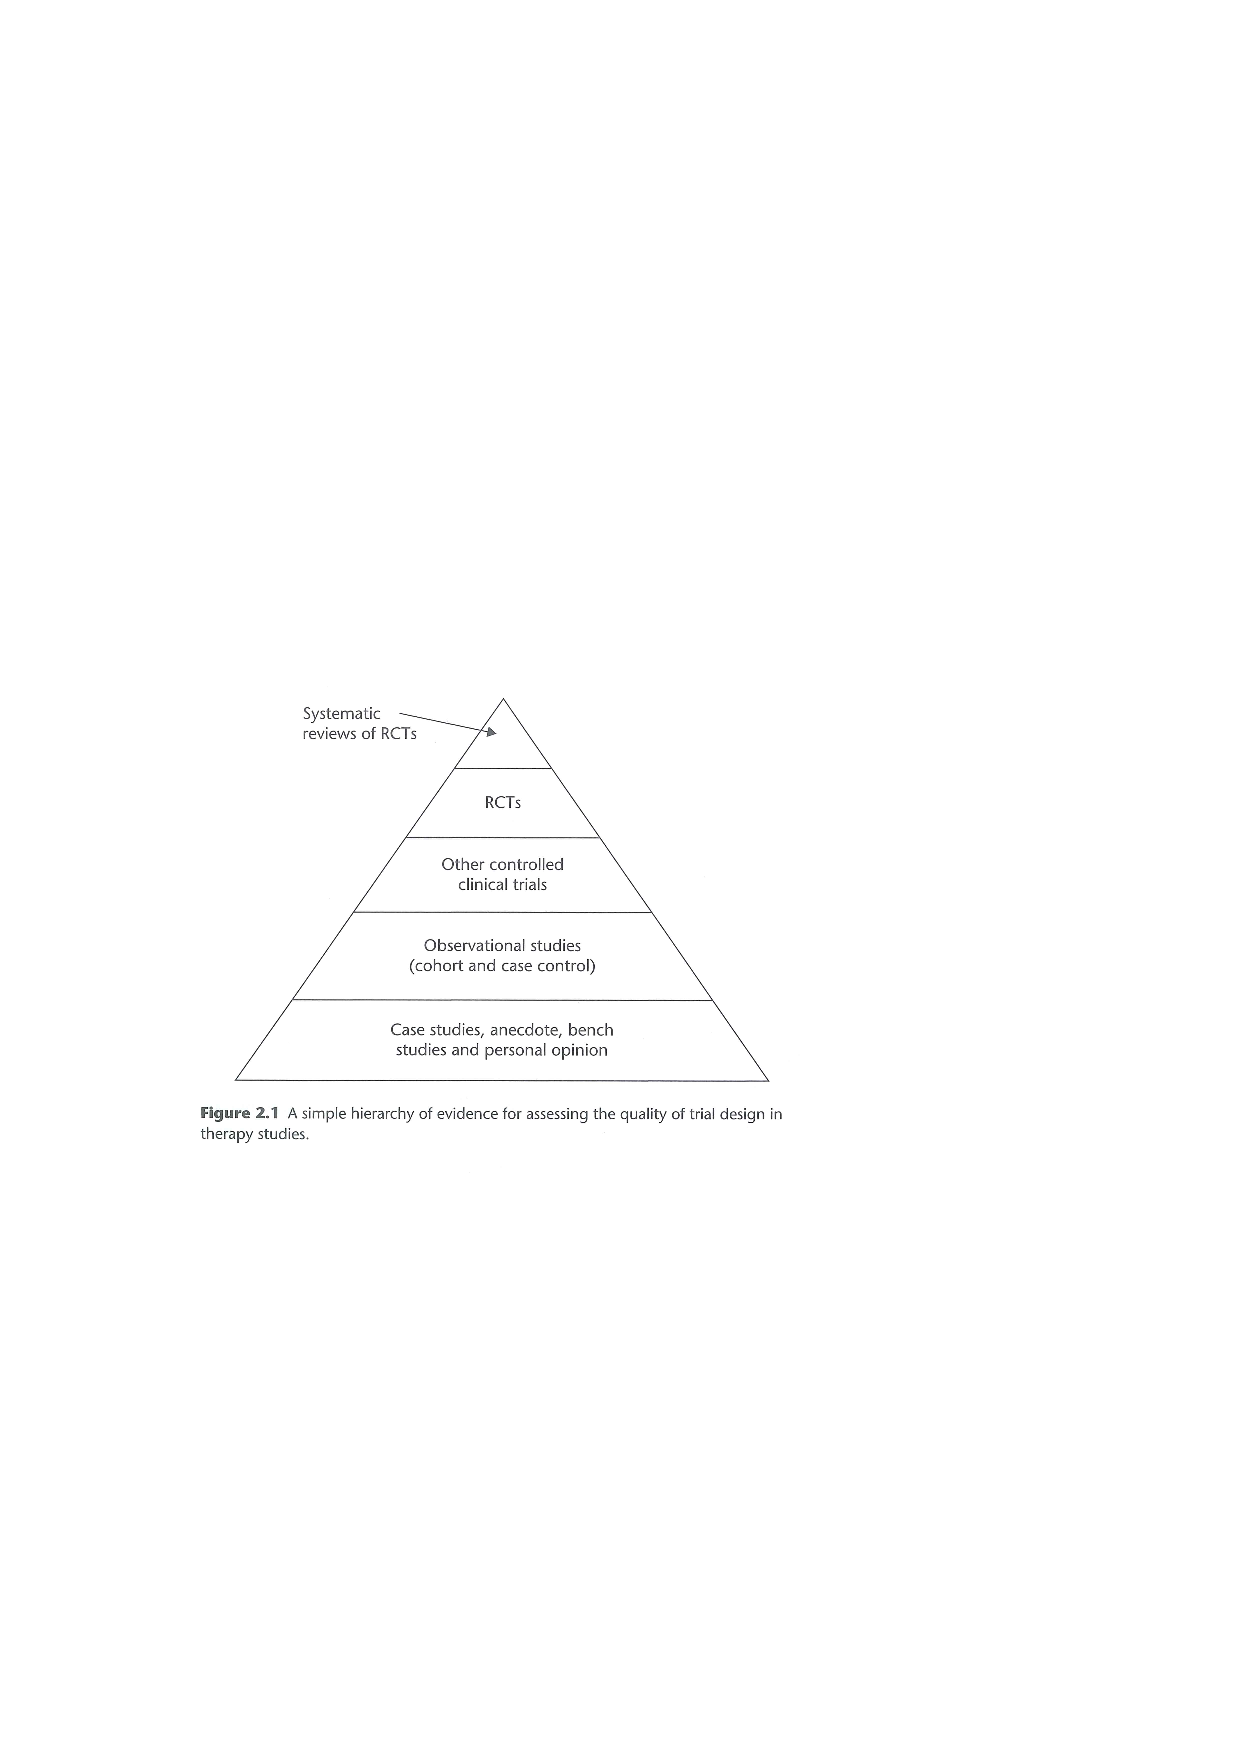
\includegraphics[width=.9\textwidth]{images/evidence_hierarchy_greenhalgh_4th.pdf}
	\end{center}
\end{frame}

%
\begin{frame}{Critically appraising case studies}
	\begin{itemize}
	\item Available at University of Adelaide's Joanna Briggs Institute
	\item See \url{http://joannabriggs.org/research/critical-appraisal-tools.html}
	\end{itemize}
\end{frame}

\section*{Single-Subject Designs}

%
\begin{frame}
\center{\Huge{\textcolor{darkgray}{Single-Subject Designs}}}
\end{frame}

% 
\begin{frame}{Judging intervention effectiveness}
Two questions to ask:
	\begin{enumerate}
	\item Was there a change?
	\item Was the change due to intervention?
	\end{enumerate}
\end{frame}

% 
\begin{frame}{Single-subject designs}
	\begin{itemize}
	\item Unlike case studies, these are \textbf{experimental} rather than observational designs. 
	\item Far more convincing in terms of demonstrating intervention effectiveness since experimental control is built in.
	\item Minimum of one client needed, but most studies have more than one, since replicated evidence is always more convincing than evidence from a single client.
	\item Also known as \emph{single-subject experimental designs (SSED)} or simply, \emph{single-subject data (SSD)}
	\item Can offer a practical approach to objectively judging whether intervention works in everyday clinical settings
	\end{itemize}
\end{frame}

% 
\begin{frame}{Single-subject designs}
	\begin{itemize}
	\item Can be used to answer questions like:
		\begin{itemize}
		\item[-] Was the therapy approach effective?
		\item[-] How effective was the therapy (effect size)?
		\item[-] Which therapy approach was more effective/efficient?
		\end{itemize}
	\item Use data collected from one individual (or more) to establish cause-and-effect relationships
	\item Permit detailed descriptions of intervention progress in a single individual
	\item Involve observations (measurements) made repeatedly over time
	\end{itemize}
\end{frame}

% 
\begin{frame}{Example: measure behaviour \textbf{before} intervention}
	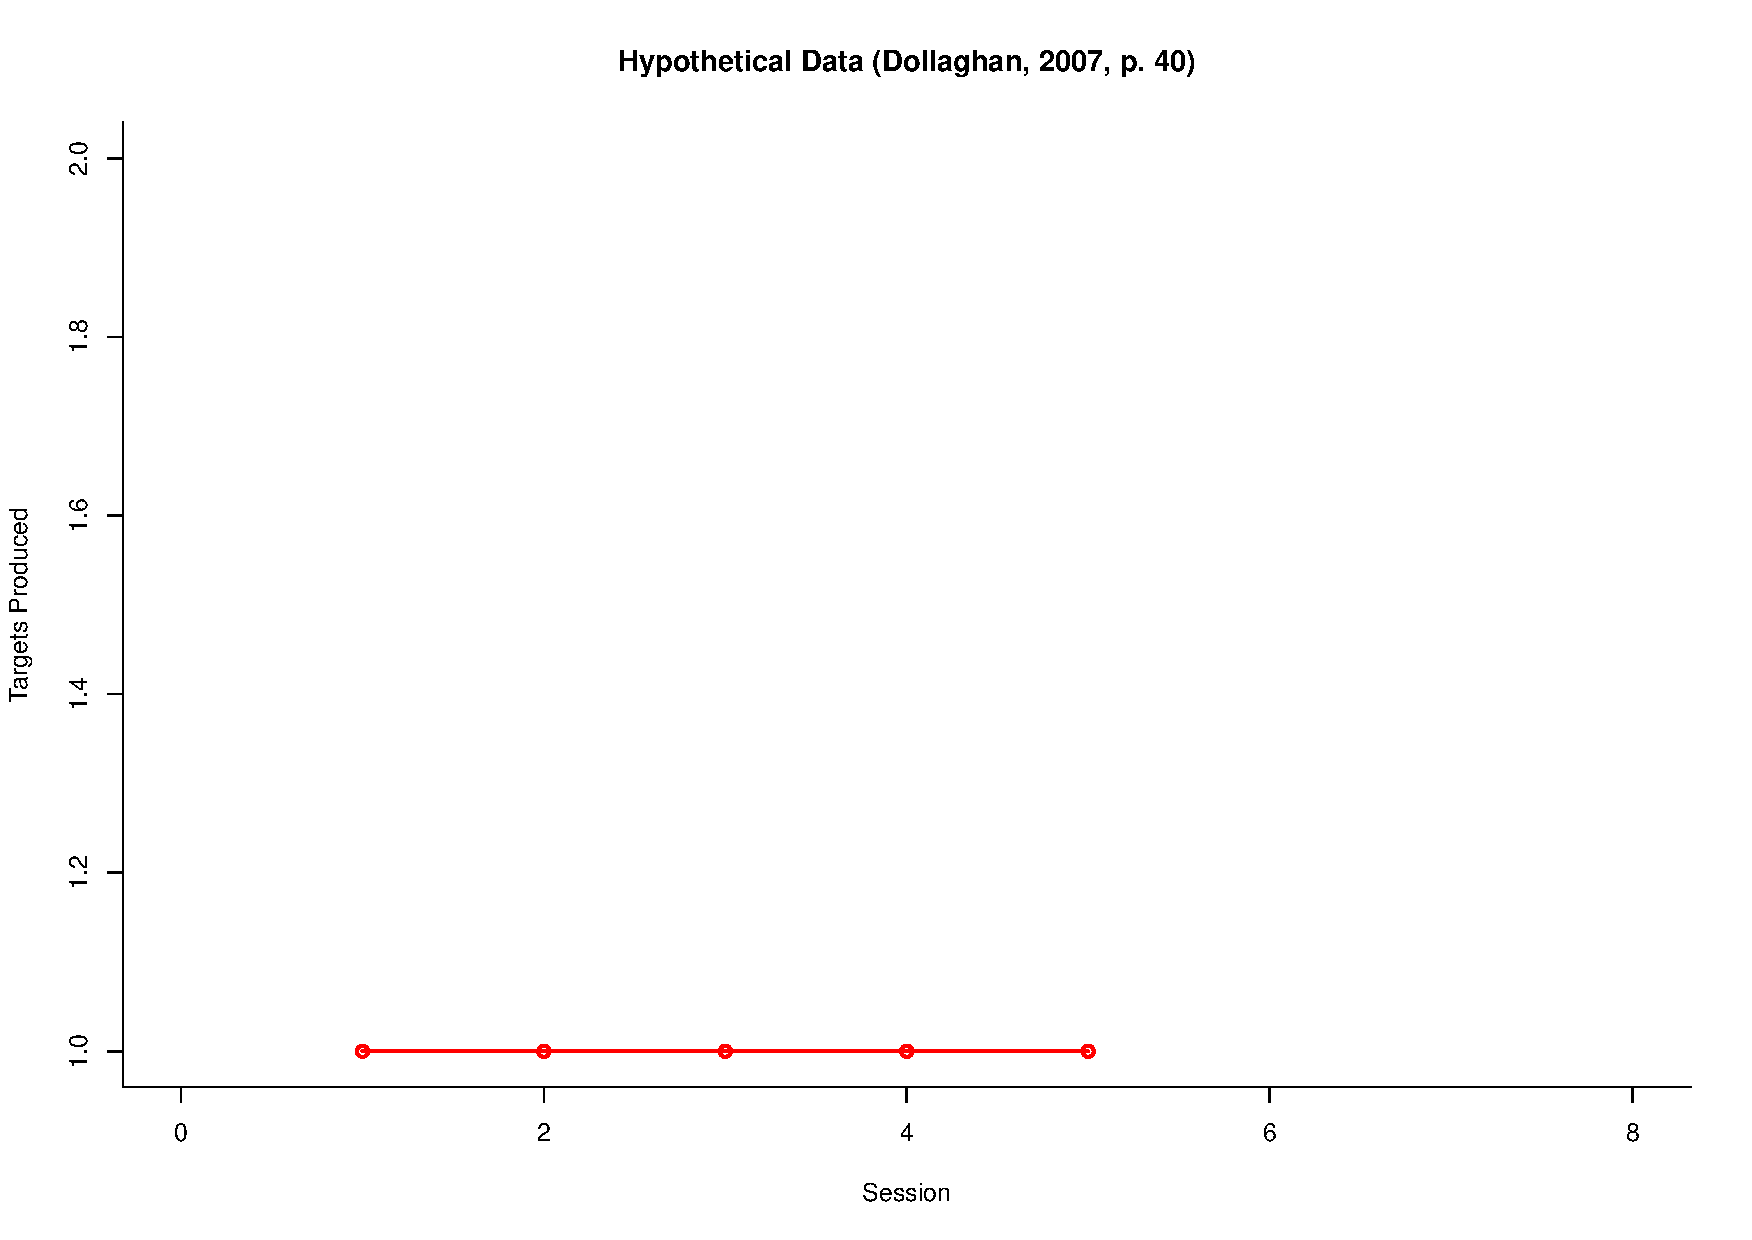
\includegraphics[width=10cm]{SSD/Aplot.pdf}
\end{frame}

% 
\begin{frame}{Example: measure behaviour \textbf{during} intervention}
%	\begin{center}
	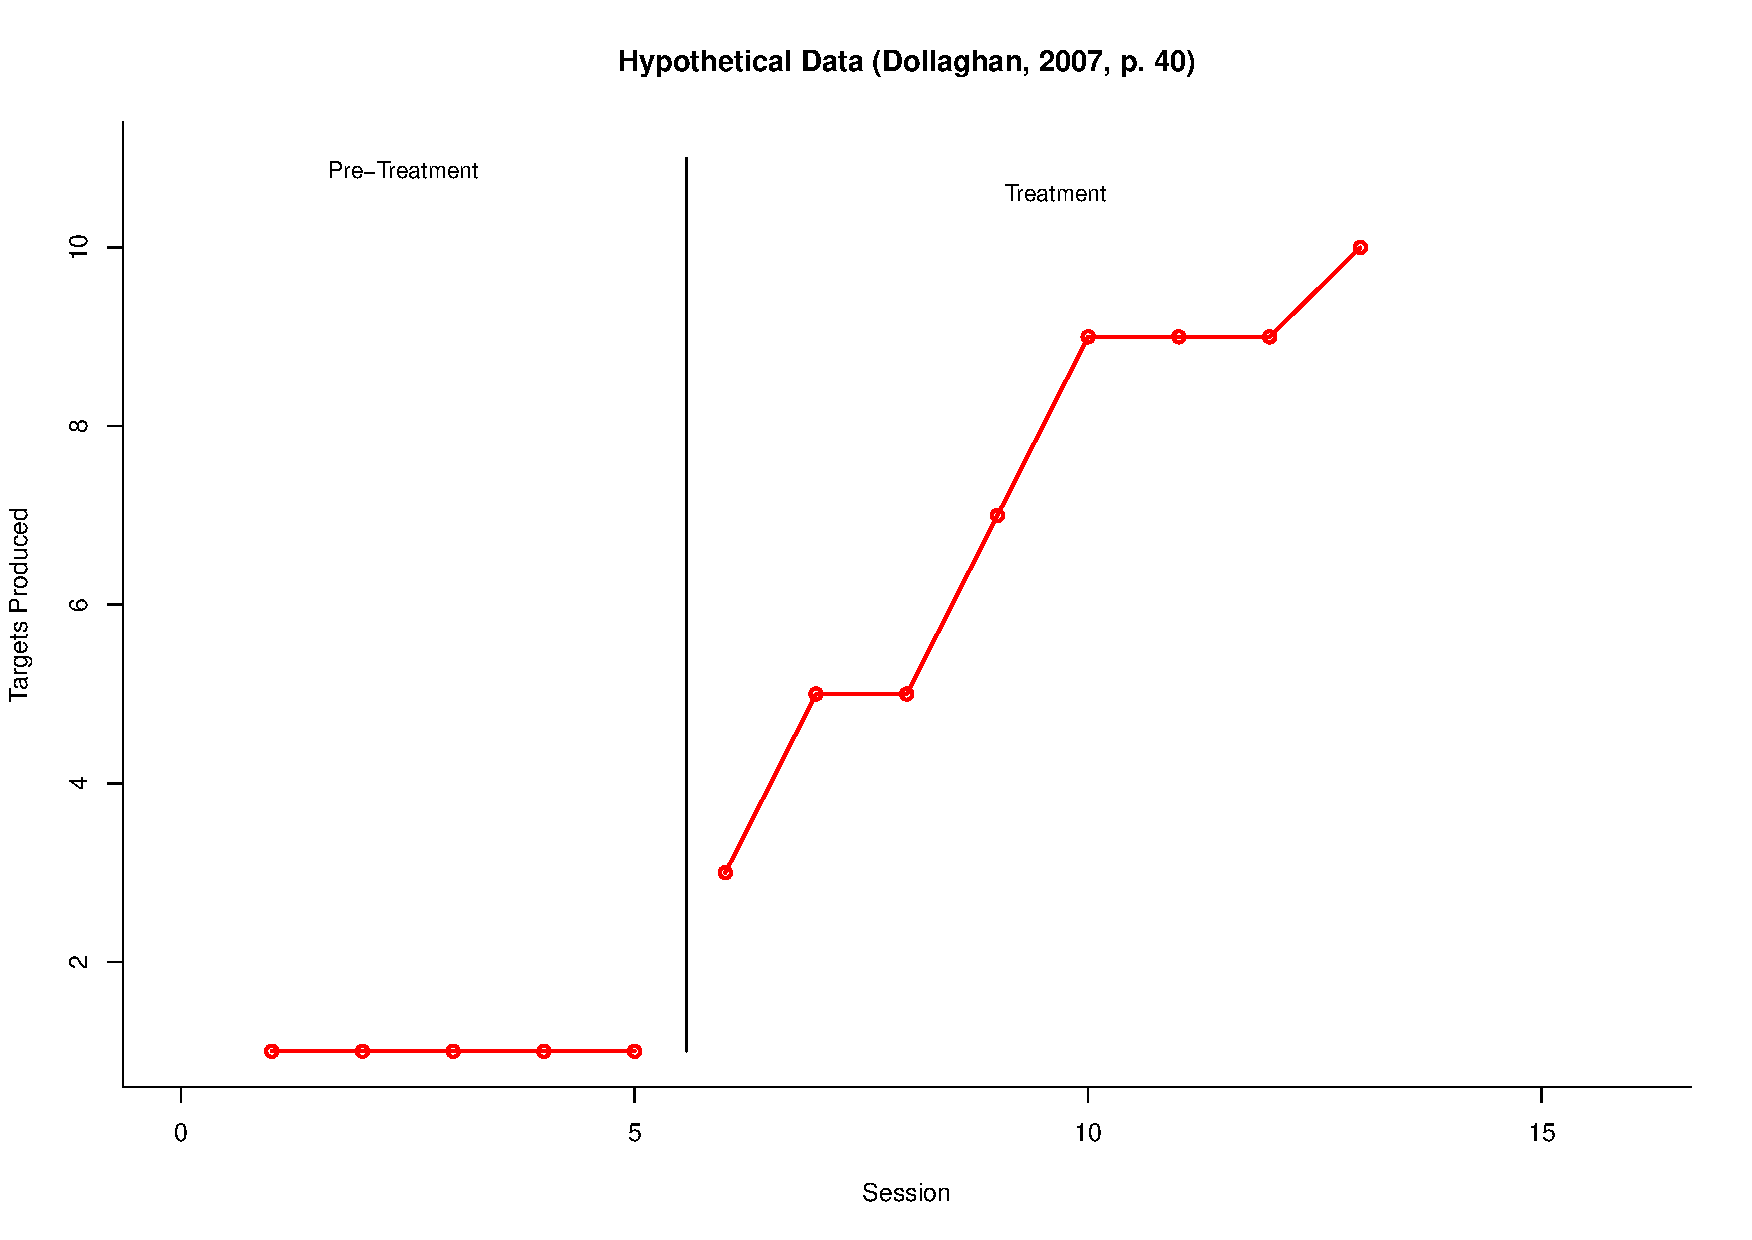
\includegraphics[width=10cm]{SSD/ABplot.pdf}
%	\end{center}
\end{frame}

% 
\begin{frame}{Single-subject design features}
	\begin{itemize}
	\item \textbf{Independent variable:} the variable being manipulated by the investigator
	\item Examples: intervention vs no invention; type of intervention provided; type of feedback provided during intervention; type of stimuli (e.g. phonemic vs semantic) used during intervention (e.g. for word retrieval); intensity of intervention
	\end{itemize}
\end{frame}

% 
\begin{frame}{Single-subject design features}
	\begin{itemize}
	\item \textbf{Dependent variable:} the variable being measured---the thing you think will change if intervention works.
	\item Examples: number or percentage of items correct on a \textbf{probe} task; number of behaviours observed; number of times child displays aggressive behaviour; heart-rate; blood pressure
	\end{itemize}
\end{frame}

% 
\begin{frame}{Probe tasks}
	\begin{itemize}
	\item A \textbf{stable pre-treatment baseline} is essential. One rule-of-thumb: stability means 3 baseline probes that don't differ by more than 10\%.
	\item Consider timing of probe tasks.
		\begin{itemize}
		\item[-] What's measured if they're done at the end of each session? 
		\item[-] At the beginning?
		\end{itemize}
	\item Consider randomly selecting probe items from a larger item-pool each time the probe task is given. This offers more experimental control than using the same items each time to indicate that learning has taken place.
	\item Probe task doesn't have to be administered each session.
	\end{itemize}
\end{frame}

% 
\begin{frame}{SSD phases}
	\begin{itemize}
	\item All SSDs consist of \textbf{phases}. A phase is a series of observations of the same individual under the same conditions.
	\item A \textbf{baseline phase} refers to a no-treatment period (\textbf{{``A" phase}}).  
	\item A \textbf{treatment phase} refers to an intervention period (\textbf{{``B" phase}}).
	\item Some designs may involve a comparison with another intervention (\textbf{{``C" phase}}).
	\end{itemize}
\end{frame}

% 
\begin{frame}{A simple AB design}
	\begin{center}
	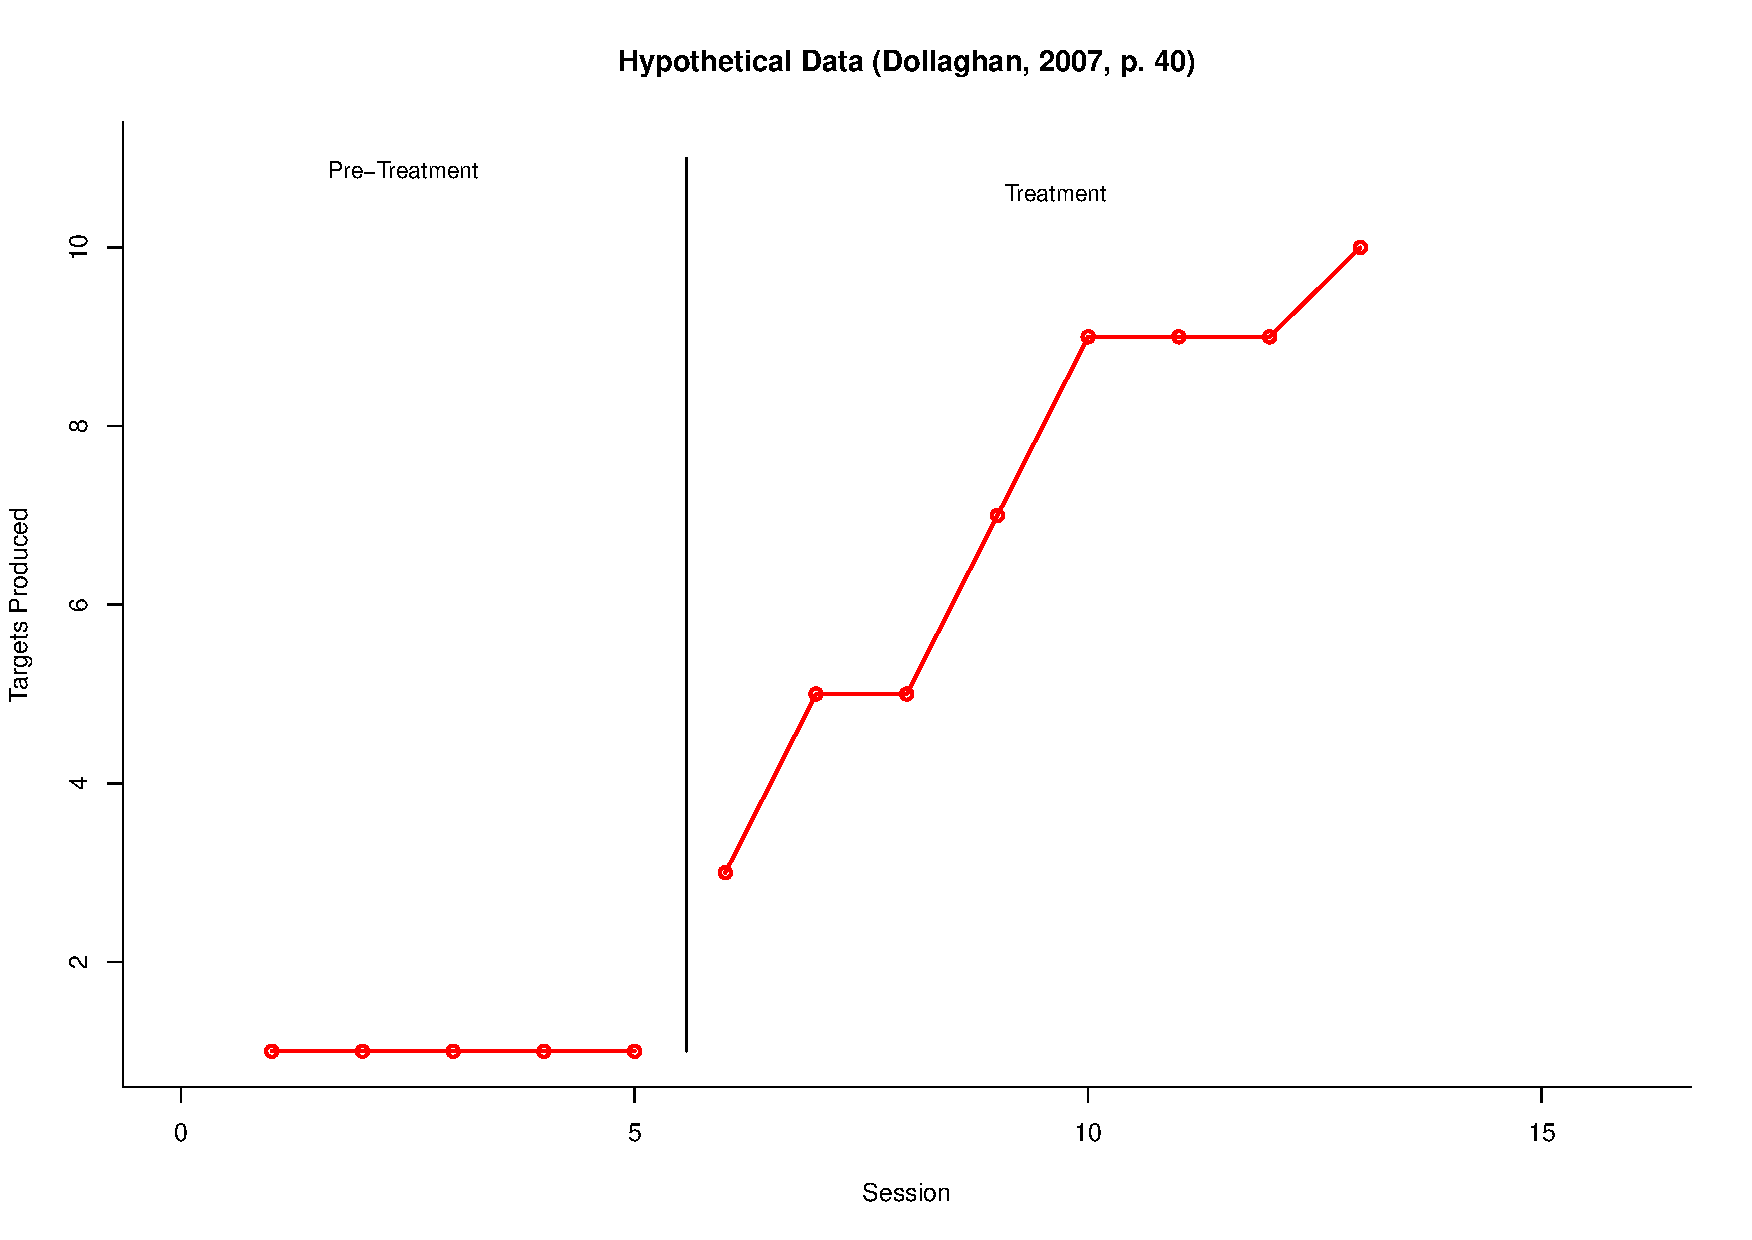
\includegraphics[width=10cm]{SSD/ABplot.pdf}
	\end{center}
\end{frame}

% 
\begin{frame}{Judging intervention effectiveness}
Let's ask those two questions again:
	\begin{enumerate}
	\item Was there a change?
	\item Was the change due to intervention?
	\end{enumerate}
\end{frame}

% 
\begin{frame}{More powerful kinds of SSDs}
	\begin{itemize}
	\item Withdrawal (reversal) design (ABA)
	\item Multiple baseline designs
		\begin{itemize}
		\item[-] across behaviours
		\item[-] across settings
		\item[-] across subjects
		\end{itemize}
	\item Alternating treatment design (ATDs)
	\end{itemize}
\end{frame}

% 
\begin{frame}{Data analysis and interpretation}
	\begin{itemize}
	\item By visually interpreting the data
		\begin{itemize}
		\item[-] Look for a change in the slope of the data points between phases.
		\item[-] Then plot the data without indicating where the phase changed.
		\item[-] Ask another person to indicate where on the x-axis the slope changes.
		\item[-] Compare these to the actual location of the phrase change. 
		\item[-] It's unrealistic to expect improvement on the probe task as soon as treatment phase begins. Learning often takes longer than that!
		\item[-] \textbf{Replication} is important (a drawback of the AB design).
		\end{itemize}
	\item By statistical analysis (next session)
	\end{itemize}
\end{frame}

% 
\begin{frame}{Evidence quality\footnote{\tiny{\citet{Guyatt2008d}}}}
	\begin{itemize}
	\item \alert{N-of-1 randomized trial}
	\item SR of randomized trials
	\item Single randomized trial
	\item SR of observational studies addressing patient-important outcomes
	\item Single observational study addressing patient-important outcomes 
	\item Physiological studies (studies of blood pressure, cardiac output, etc.)
	\item Unsystematic clinical observations
	\end{itemize}
\end{frame}

\begin{frame}{Evidence quality}
	\begin{itemize}	
	\item \citet[p. 40]{Dollaghan2007a} noted that \citet{Guyatt2000} ``placed the N-of-1 randomized trial at the top of their evidence hierarchy for making treatment decisions about a particular patient.''
	\item Think about why that might be so. 
	\item \emph{Hint:} How do SSDs compare to RCTs?
	\item What advantages might these have over RCTs?
	\end{itemize}
\end{frame}

\section*{Group Discussion}

% 
\begin{frame}{Group discussion}
	\begin{itemize}
	\item Break up into your assigned groups.
	\item Critically appraise today's research using the SCED (\url{http://www.psycbite.com/docs/The_SCED_Scale.pdf}).
	\item For description of SCED items, see \citet[pp. 400--401]{Tate2008}. 
	\item Document on the form \emph{where} you found information in the research article addressing each point.
	\end{itemize}
\end{frame}

\begin{frame}[shrink=15] % to reduce font size of references
	\frametitle{References}
	\bibliographystyle{apacite}
	\small\bibliography{/Users/thomasklee/Documents/Bibtex/library}
 \end{frame}

\end{document}